% ADD THIS HEADER TO ALL NEW CHAPTER FILES FOR SUBFILES SUPPORT

% Allow independent compilation of this section for efficiency
\documentclass[../CLthesis.tex]{subfiles}

% Add the graphics path for subfiles support
\graphicspath{{\subfix{../images/}}}

% END OF SUBFILES HEADER

%%%%%%%%%%%%%%%%%%%%%%%%%%%%%%%%%%%%%%%%%%%%%%%%%%%%%%%%%%%%%%%%
% START OF DOCUMENT: Every chapter can be compiled separately
\begin{document}

\chapter{Experiment 2: Token-based Deep Learning Methods}%
% \label{chap:experiment_2}
\refstepcounter{experiment}  % This increments the counter
\label{exp:\theexperiment}
This experiment aimed to process neural data using NLP methods. The spike data were converted into text tokens in the NLP framework.

\section{Methods}
\subsection{Tokenization Method}
We passed in binary data in a text format. For each sampling time, the data were then combined across all 75 neurons from the shallowest to the deepest. For binary data, each value was either 1, which indicates a firing, or 0, which indicates non-existence of firing. Each text token would then be composed of $75$ binary values. Data representing one sampling time ($0.05$\,ms) is shown below:

\begin{equation*}
\underbrace{\texttt{<|START|>}}_{\texttt{bos}}\underbrace{\texttt{0000100000...0000000010}}_{75\text{ Neurons}}\underbrace{\texttt{<|END|>}}_{\texttt{eos}}
\end{equation*}

The first 0 refers to neuron 1 being inactive, and fifth 1 refers to neuron 5 being active. The neurons are re-indexed according to their depth to probe tip from small to large. 

We collected all such combinations, and used Byte-Pair Encoding (BPE) to train a tokenizer. The goal was to represent each sampling time by one input token ID. Since BPE creates both complete units and subunits with varying lengths, we aimed to keep only complete tokens with a length of $75$ (which is equal to the number of neurons). Since the tokenizer was trained on all possibilities, it automatically prioritized single complete tokens over multiple subunit combinations. Thus in practice, the incomplete subtokens had no impact on performance and were kept in the vocabulary. Figure~\ref{fig:tokens} shows how the data were tokenized.
\begin{figure}[H]
% \begin{center}
\centering
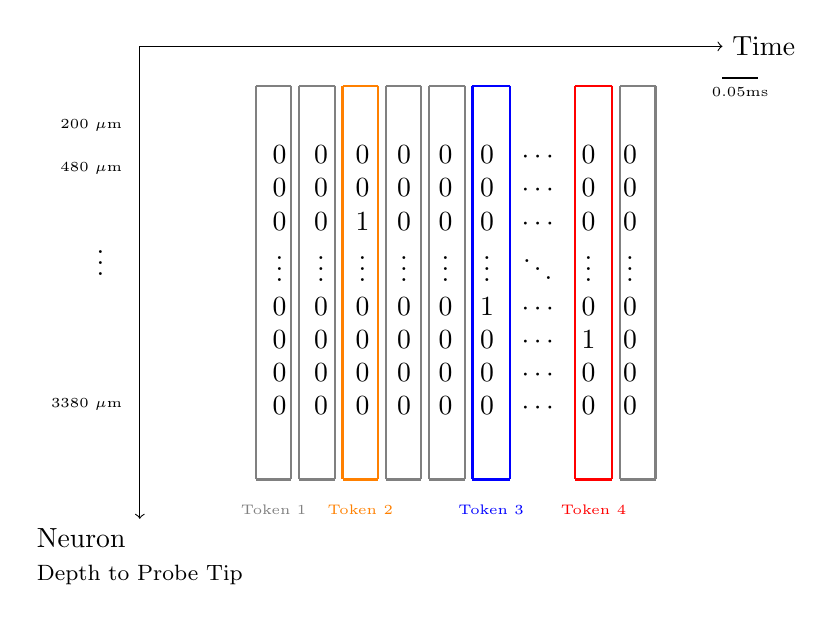
\begin{tikzpicture}
% Time arrow on top
\draw[->] (0,0) -- (7.4,0) node[right, align=left] {Time};

% Add the scale bar and label at the end of time axis (7.2)
\draw[thick] (7.4,-0.4) -- (7.85,-0.4);
\node[anchor=north] at (7.625,-0.4) {\tiny 0.05ms};

% Neuron arrow on left with labels
\draw[->] (0,0) -- (0,-6) node[below, align=left] {Neuron\\{\footnotesize Depth to Probe Tip}};

% Add y-axis labels
\node[anchor=east] at (-0.1,-1.0) {\tiny 200 $\mu$m};  % 0 micrometer at top
\node[anchor=east] at (-0.1,-1.55) {\tiny 480 $\mu$m};  % 0 micrometer at top
\node[text=black] at (-0.5,-2.65) {$\vdots$};  % Add vertical dots in the middle
\node[anchor=east] at (-0.1,-4.55) {\tiny 3380 $\mu$m};  % 3500 micrometer in middle

    % Binary data matrix
    \node at (4,-3) {$\begin{array}{ccccccccc}
        0 & 0 & 0 & 0 & 0 & 0 & \cdots & 0 & 0\\
        0 & 0 & 0 & 0 & 0 & 0 & \cdots & 0 & 0\\
        0 & 0 & 1 & 0 & 0 & 0 & \cdots & 0 & 0\\
        \vdots & \vdots & \vdots & \vdots & \vdots & \vdots & \ddots & \vdots & \vdots \\
        0 & 0 & 0 & 0 & 0 & 1 & \cdots & 0 & 0\\
        0 & 0 & 0 & 0 & 0 & 0 & \cdots & 1 & 0\\
        0 & 0 & 0 & 0 & 0 & 0 & \cdots & 0 & 0\\
        0 & 0 & 0 & 0 & 0 & 0 & \cdots & 0 & 0\\
    \end{array}$};


% first column	
\draw[black!50, thick] (1.475,-0.5) -- (1.475,-5.5);
\draw[black!50, thick] (1.925,-0.5) -- (1.925,-5.5);
\draw[black!50, thick] (1.475,-0.5) -- (1.925,-0.5);
\draw[black!50, thick] (1.475,-5.5) -- (1.925,-5.5);

% Second column - black!50
\draw[black!50, thick] (2.025,-0.5) -- (2.025,-5.5);
\draw[black!50, thick] (2.475,-0.5) -- (2.475,-5.5);
\draw[black!50, thick] (2.025,-0.5) -- (2.475,-0.5);
\draw[black!50, thick] (2.025,-5.5) -- (2.475,-5.5);

% Third column - orange
\draw[orange, thick] (2.575,-0.5) -- (2.575,-5.5);
\draw[orange, thick] (3.025,-0.5) -- (3.025,-5.5);
\draw[orange, thick] (2.575,-0.5) -- (3.025,-0.5);
\draw[orange, thick] (2.575,-5.5) -- (3.025,-5.5);

% Fourth column - black!50
\draw[black!50, thick] (3.125,-0.5) -- (3.125,-5.5);
\draw[black!50, thick] (3.575,-0.5) -- (3.575,-5.5);
\draw[black!50, thick] (3.125,-0.5) -- (3.575,-0.5);
\draw[black!50, thick] (3.125,-5.5) -- (3.575,-5.5);

% Fifth column - black!50
\draw[black!50, thick] (3.675,-0.5) -- (3.675,-5.5);
\draw[black!50, thick] (4.125,-0.5) -- (4.125,-5.5);
\draw[black!50, thick] (3.675,-0.5) -- (4.125,-0.5);
\draw[black!50, thick] (3.675,-5.5) -- (4.125,-5.5);

% Sixth column - blue
\draw[blue, thick] (4.225,-0.5) -- (4.225,-5.5);
\draw[blue, thick] (4.7,-0.5) -- (4.7,-5.5);
\draw[blue, thick] (4.225,-0.5) -- (4.7,-0.5);
\draw[blue, thick] (4.225,-5.5) -- (4.7,-5.5);

% Penult column - red
\draw[red, thick] (5.525,-0.5) -- (5.525,-5.5);
\draw[red, thick] (6.0,-0.5) -- (6.0,-5.5);
\draw[red, thick] (5.525,-0.5) -- (6.0,-0.5);
\draw[red, thick] (5.525,-5.5) -- (6.0,-5.5);

% Last column - black!50
\draw[black!50, thick] (6.1,-0.5) -- (6.1,-5.5);
\draw[black!50, thick] (6.55,-0.5) -- (6.55,-5.5);
\draw[black!50, thick] (6.1,-0.5) -- (6.55,-0.5);
\draw[black!50, thick] (6.1,-5.5) -- (6.55 ,-5.5);

% Token labels
\node[anchor=north] at (1.7,-5.7) {\textcolor{black!50}{\tiny Token 1}};
\node[anchor=north] at (2.8,-5.7) {\textcolor{orange}{\tiny Token 2}};
\node[anchor=north] at (4.4625,-5.7) {\textcolor{blue}{\tiny Token 3}};
\node[anchor=north] at (5.7625,-5.7) {\textcolor{red}{\tiny Token 4}};
    
\end{tikzpicture}
% \end{center}
\caption{Transforming neural data in sampling time into tokens}
\label{fig:tokens}
\end{figure}

We then used this tokenizer to tokenize the whole data, and we added three special tokens: (1) begin of sequence (bos) token \texttt{<|START|>}, (2) end of sequence (eos) token \texttt{<|END|>}, and (3) divider \texttt{<|>}. The divider \texttt{<|>} was used to combine multiple sampling times together. A data for two sampling times (0.1\,ms) combined together looks like:
\begin{equation*}
\texttt{<|START|>}\underbrace{\texttt{0000100000...0000000010}}_{\text{ Data 1}}\underbrace{\texttt{<|>}}_{\text{divider}}\underbrace{\texttt{0000000000...0010000000}}_{\text{Data 2}}\texttt{<|END|>}
\end{equation*}

This tokenization method allowed us to represent binary spike train data into limited numbers of tokens for subsequent analysis. The obtained vocabulary size is $4087$ ($7107$ including subunits), and $\approx$ 90\,\% of the data is empty data consisting of 75 zeros.

\subsection{Data preparation} 
We used the following data lengths: 0.05\,ms (with and without empty tokens), 0.5\,ms, 1.5\,ms, 2.5\,ms, 3\,ms, 5\,ms, 6\,ms, 15\,ms, 30\,ms, 45\,ms, and 60\,ms. Since 60\,ms exceeded the lengths of some annotated syllables, padding was introduced to maintain consistent input dimensionalities. 
\subsection{Models and Evaluation} 
We randomly initialized the weights of two Hugging Face models to borrow their mature structures. The first model is OpenAI GPT-2 model \citep{Radford2019-gx} with 142M parameters, and the second model is a Mamba \citep{Gu2023-vw} model with 130M parameters with a sequence classification head. The models were evaluated using classification accuracies across different data lengths and model architectures. We then compared the best performing model against our previously established SVM benchmark.
\section{Results}
\subsection{GPT-2 performance}
Table~\ref{tab:gpt2_performance} and Figure~\ref{fig:GPT} show the classification accuracy of GPT-2 increases with input data length from 15\,ms, and reaches 47\,\% with information from 60\,ms. On the other hand, data shorter than 15\,ms failed for the task, even when the sparsity was removed.
\begin{figure}[htbp]
    \centering
    \includegraphics[width=0.8\textwidth]{images/gpt_performance.pdf}
    \caption{Performance of GPT-2}
    \label{fig:GPT}
\end{figure}
\begin{table}[htbp]
\centering
\begin{tabular}{cc}
\toprule
Time (ms) & Accuracy (\%) \\
\midrule
15.0 & 38.5 \\
30.0 & 41.6 \\
45.0 & 44.8 \\
\mathBF{60.0} & \mathBF{47.0} \\
\bottomrule
\end{tabular}
\caption{GPT-2 classification accuracy with sequences from 15\,ms to 60\,ms}
\label{tab:gpt2_performance}
\end{table}

\subsection{Mamba performance}
Figure~\ref{fig:MambaText} shows that Mamba 130M failed the task with sequence length 45\,ms.
\begin{figure}[H]
    \centering
    \includegraphics[width=0.8\textwidth]{images/result_mamba_900.pdf}
    \caption{Mamba confusion matrix with 45\,ms sequences}
    \label{fig:MambaText}
\end{figure}

\section{Discussion}
\subsection{Achievements on GPT-2 performance}
Figure~\ref{fig:GPT} shows the potential of GPT-2 in neural decoding tasks. The performance of the model increases to 47.0\,\% with longer input sequence length. Our findings demonstrate the validity of the approach for transformers to deal with neural data as text tokens. 
\subsection{Limitations}
The performance of GPT-2 model is not optimal. The final accuracy of 47\,\% is below our established SVM benchmark 77.3\,\% using mean firing rates. Additionally, the small Mamba model failed to decode $45$\,ms length data. The performance of large language models indicate that more data is needed.

\subsection{Future Directions}
The current decoding accuracy can be improved by training with data from the motor pathway instead of AFP. In addition, a pre-trained model could be developed using synthesized \citep{Zhou2020-om} or open \citep{de-Vries2020-ld} data from other animals and experiment paradigms, and then fine-tuned using real vocalization data. Introducing mixed transformer-mamba layers \citep{Lieber2024-hk} is also a promising approach to enhance the decoding accuracy.



% self-defined macro: include bibliography even when compiling a single chapter
\subfilebibliography
\end{document}
